

\section{Ziel}
In diesem Versuch werden die charakteristischen Funktionsweisen des Geiger-Müllerzählrohres überprüft sowie die Totzeit des Zählrohres bestimmt.

\section{Theorie}
\subsection{Aufbau und Funktionsweise des Geiger-Müller-Zählrohrs}
\begin{figure}[H] 
  \centering 
  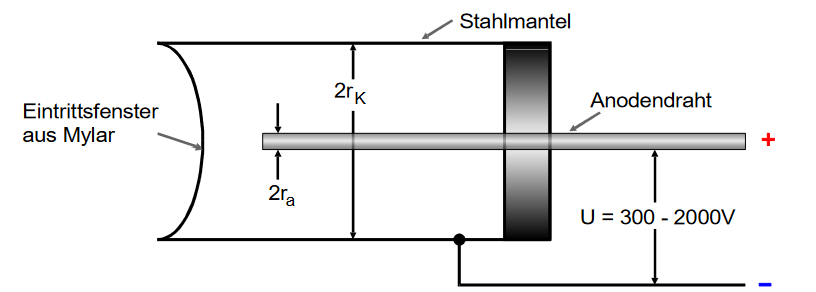
\includegraphics[width=9cm]{content/1.png} 
  \caption{Skizze des Geiger-Müller-Zählrohrs. \cite{sample}} \label{fig:1} 
\end{figure}
Das Geiger-Müller-Zählrohr besteht aus einem Kathodenzylinder, einem axial verlaufenden Anodendraht und aus einem Eintrittsfenster aus Mylar. Das Zählrohr ist mit einem Gasgemisch aus Argon und Ethylaklohol gefüllt. Wird eine äußere Spannung an das Zählrohr angelegt, entsteht ein Feld, in dem ein geladenes Teilchen fließen kann. Dieses Teilchen kann durch Ionisationsakte absorbiert werden, wobei die Anzahl an entstehenden Elektronen und positiven Ionen proportional zu Energie des einfallenden Teilchens ist. Die nach der Primärionisation ablaufenden Vorgänge sind stark von der angelegten Spannung abhängig.\\
\begin{figure}[H] 
  \centering 
  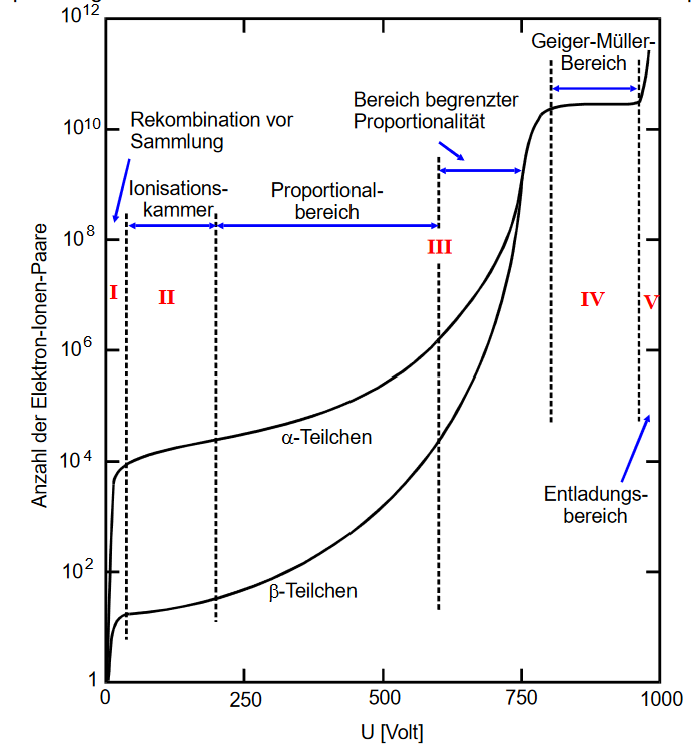
\includegraphics[width=9cm]{content/2.png} 
  \caption{Bereiche des Geiger-Müller-Zählrohrs \cite{sample}.} \label{fig:2} 
\end{figure}

Bei geringer Spannung erreicht nur ein kleiner Teil der neuen Elektronen den Draht und der Rest geht verloren. Das entspricht Teil I in \autoref{fig:2}.\\ 
Bei etwas mehr Spannung, wie im Bereich von II aus \autoref{fig:2}, erreichen alle erzeugten Elektronen den Draht und der Ionisationsstrom der zwischen Kathode und Anode fließt ist proportional zur Energie und Intensität der einfallenden Strahlung. Es können allerdings in dieser Ionisationskammer nur hohe Strahlintensitäten gemessen werden.\\
Im Spannungsbereich von Teil III aus \autoref{fig:2} können die freien Elektronen die Argon-Atome ionisieren. Bei der Stoßionisation können die neu freigesetzten Atome wieder ioniseren. Es folgt also eine Lawine an ionisationen, die auch Townsend-Lawine genannt wird. Die Ladung $Q$ ist jetzt so groß, dass sie gemessen werden kann, was von Vorteil ist, da sie proportional zur Energie ist. Neben der Strahlintensität kann also auch die Energie gemessen werden. \\
Liegt die äußere Spannung im Bereich IV aus \autoref{fig:2}, dann werden zusätzlich zu den Elektronen auch Photonen freigesetzt, weshalb nur noch die Intensität gemessen werden kann. Dieser Bereich heißt auch Wirkungsbereich und ist der eigentliche Arbeitsbereich des Geiger-Müller-Zählrohrs [1].

\subsection{Totzeit}
Weil die positiven Ionen massereicher als die Elektronen sind, brauchen sie länger, um durch den Anodendraht aus dem Zählrohr zu verschwinden. Durch ihr längeres Verweilen schwächt sich das elektrische Feld für eine Zeit $T$ ab, sodass die durch die Ionisation entstandenen Ionen nicht bis zur Anode beschleunigt werden. Diese Zeit $T$ heißt auch Totzeit. Nach der Totzeit folgt die Erholungszeit $T_E$, die als Zeitraum definiert ist, in der die Ausgangsimpulse eine geringere Amplitude haben. Das Ganze wird noch einmal in \autoref{fig:3} dargestellt.\\
Die Totzeit kann durch die Zwei-Quellen-Methode ermittelt werden. Die gemessene Teilchenzahl $N_r$ ist immer kleiner als die wahre Teilchenzahl
\begin{equation}
  N_w=\frac{\textrm{Impulsrate}}{\textrm{Meßzeit}}=\frac{N_r}{1-TN_r}
  \label{eq:1}
\end{equation}
und durch Umstellen von \eqref{eq:1} ergibt sich die Totzeit
\begin{equation}
  T=\frac{N_1+N_2-N_{1+2}}{2N_{1}N_{2}},
  \label{eq:2}
\end{equation}
wobei $N_1$ die gemessene Teilchenzahl der ersten radioaktiven Probe, $N_2$ die der zweiten radioaktiven Probe und $N_1 + N_2$ die gemessene Teilchenzahl der beiden kombinierten Proben.
Die beiden Zeitbereiche sind in \autoref{fig:3} abgebildet \cite{sample}.
\begin{figure}[H] 
  \centering 
  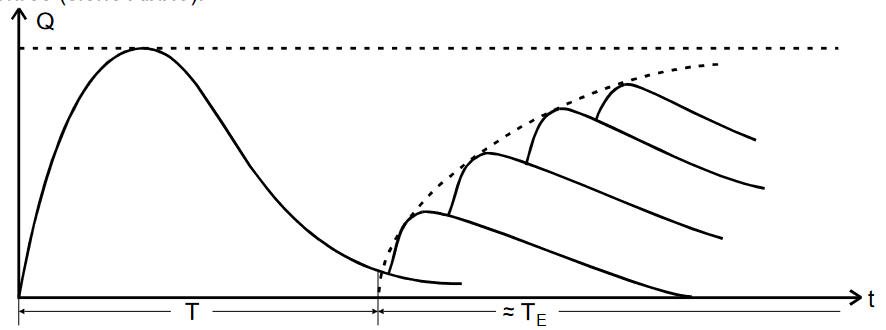
\includegraphics[width=9cm]{content/3.png} 
  \caption{Ladung gegen Zeit zur Darstellung der Tot- und Erholungszeit \cite{sample}.} 
  \label{fig:3} 
\end{figure}



\subsection{Charakteristik des Zählrohrs}
Wird die Teilchenzahl $N$ gegen die Spannung $U$ bei konstanter Strahlungsintensität aufgetragen, ergibt sich die Charakteristik des Zählrohrs. Der waagerechte bis schwach linear steigende Teil in \autoref{fig:4} heißt Plateu und ist er der Bereich des Auslösebereichs. Wird das Plateu überschritten, zerstört sich das Zählrohr im Inneren selbst durch eine Dauerentladung der Gasteilchen.  Das wird in \autoref{fig:4} dargestellt \cite{sample}.
\begin{figure}[H] 
  \centering 
  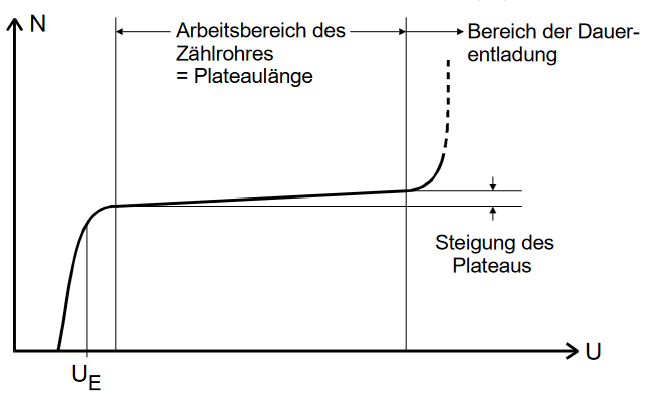
\includegraphics[width=9cm]{content/4} 
  \caption{Darstellung der Charakteristika des Zählrohrs \cite{sample}.} 
  \label{fig:4} 
\end{figure}

\subsection{Messung der freigesetzten Ladungsmenge}
Die Anzahl der freigesetzten Ladungen lässt sich durch 
\begin{equation}
  Z=\frac{I}{e_0 N}
  \label{eq:5}
\end{equation}
berechnen, wobei $I$ der Strom, $e_0$ die Elementarladung und $N$ die Impulsrate ist \cite{sample}. 
